\documentclass{standalone}
\usepackage{tikz,upgreek}
\usepackage{ctex,siunitx}
\setCJKmainfont{Noto Serif CJK SC}
\usepackage{tkz-euclide}
\usepackage{amsmath}
\usetikzlibrary{patterns, calc,3d}
\usetikzlibrary {decorations.pathmorphing,decorations.pathreplacing,decorations.shapes}
\begin{document}
\small
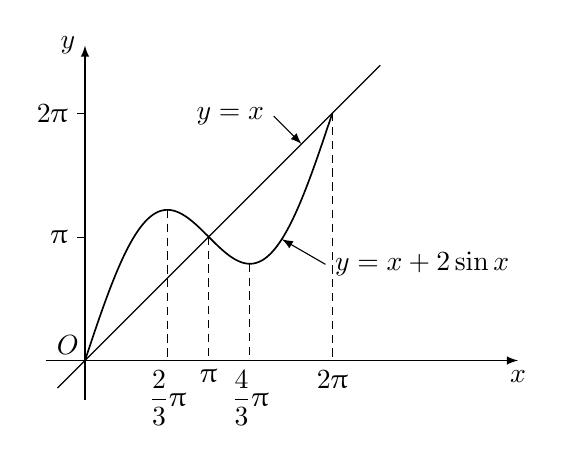
\begin{tikzpicture}[>=latex,scale=0.5]
  \draw[->](-1,0)--(11,0)node[below]{$x$};
  \draw[->](0,-1)--(0,8)node[left]{$y$};
  \draw[semithick,samples=200,domain=0:2*pi]plot(\x,{\x+2*sin(\x r)});
  \draw(-0.7,-0.7)--(7.5,7.5);
  \draw[densely dashed]({2*pi/3},{2*pi/3+sqrt(3)})--({2*pi/3},0)node[below]{$\dfrac{2}{3}\uppi$};
  \draw[densely dashed](pi,pi)--(pi,0)node[below]{$\uppi$};
  \draw[densely dashed]({4*pi/3},{4*pi/3-sqrt(3)})--({4*pi/3},0)node[below]{$\dfrac{4}{3}\uppi$};
  \draw[densely dashed](2*pi,2*pi)--(2*pi,0)node[below]{$2\uppi$};
  \draw[very thin](0,pi)--(-0.2,pi)node[left]{$\uppi$};
  \draw[very thin](0,2*pi)--(-0.2,2*pi)node[left]{$2\uppi$};
  \node at (0,0)[above left,inner sep=2pt]{$O$};
  \draw[<-](5.5,5.5)--++(135:1.0)node[left]{$y=x$};
  \draw[<-](5,{5+2*sin(5 r)})--++(-30:1.28)node[right]{$y=x+2\sin x$};
\end{tikzpicture}
\end{document}